\documentclass{article}

\usepackage{amsmath, mathtools, amsthm, tikz}

\usepackage{graphicx}
\graphicspath{ {./images/automi} }

\title{Automi}
\author{github.com/asdrubalini}
\date{\today}

\begin{document}
    \maketitle

    Automa: software generico che può funzionare su qualsiasi dispositivo programmabile.
    Un automa può essere progettato graficamente con l'utilizzo di due simboli: freccia e cerchio.
    Una volta che la progettazione è conclusa, l'automa deve essere programmato con un vero e proprio linguaggio di programmazione.

    \begin{center}
        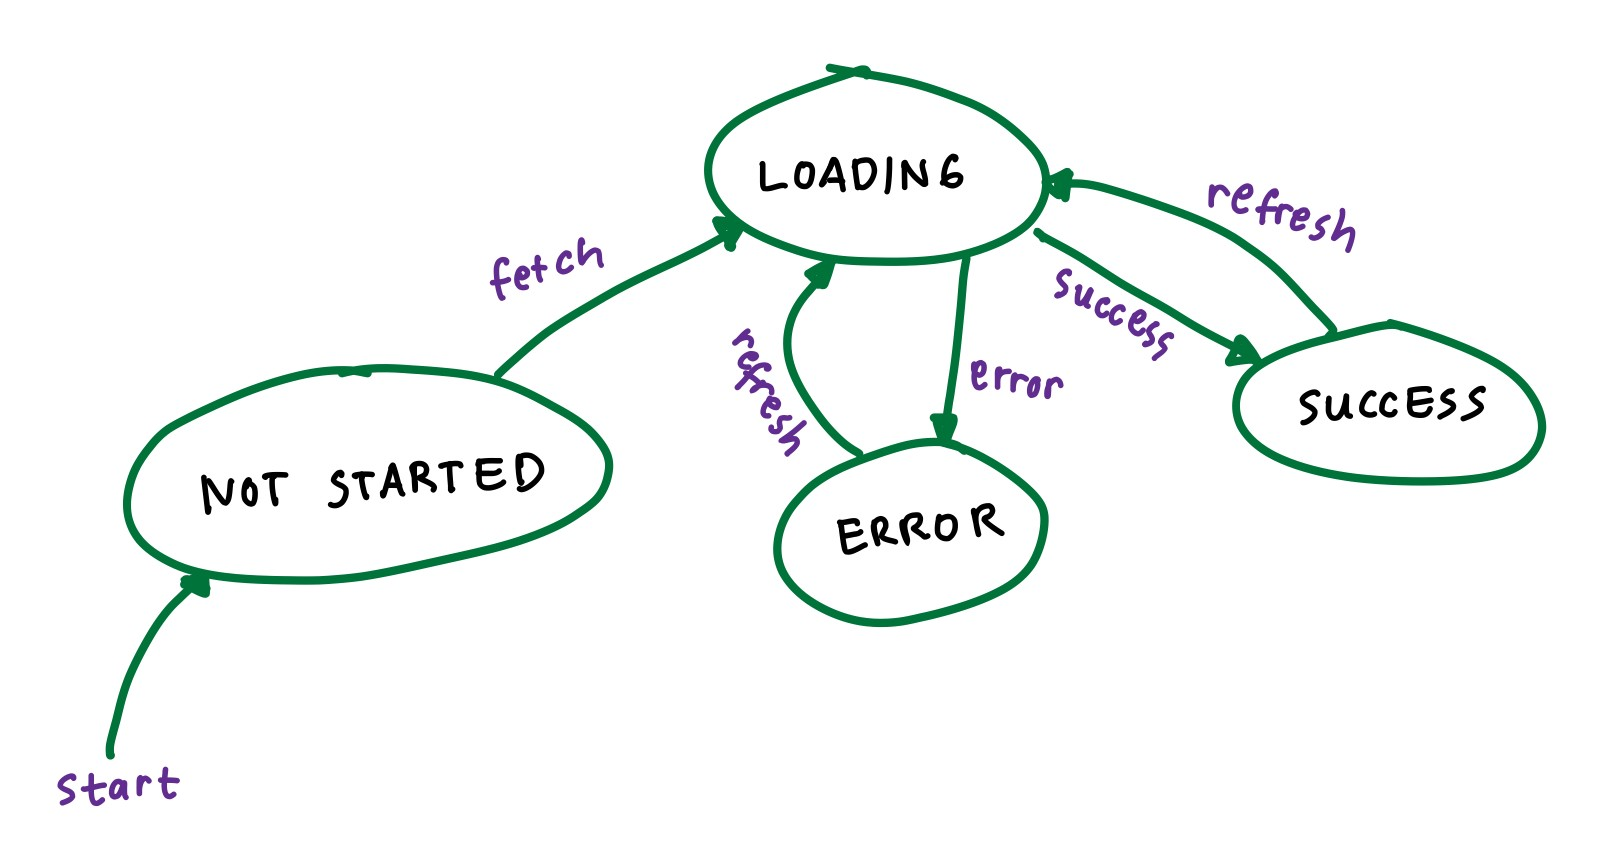
\includegraphics[width=\textwidth]{automa.png}
        esempio di diagramma che descrive un'automa
    \end{center}

    Lo stato del sistema può mutare grazie ad un evento che può essere interno (un timer) o esterno (la pressione di un bottone).
    Lo stato di partenza è essenziale, e coincide con lo stato che viene eseguito dopo l'attivazione del programma.

    \newpage

    Esercitazione: progettare l'automa che fa funzionare un semaforo.
    Verde e rosso devono avere la stessa durata (30s) mentre l'arancione deve avere un quarto della durata (7.5s). 

    \begin{center}
        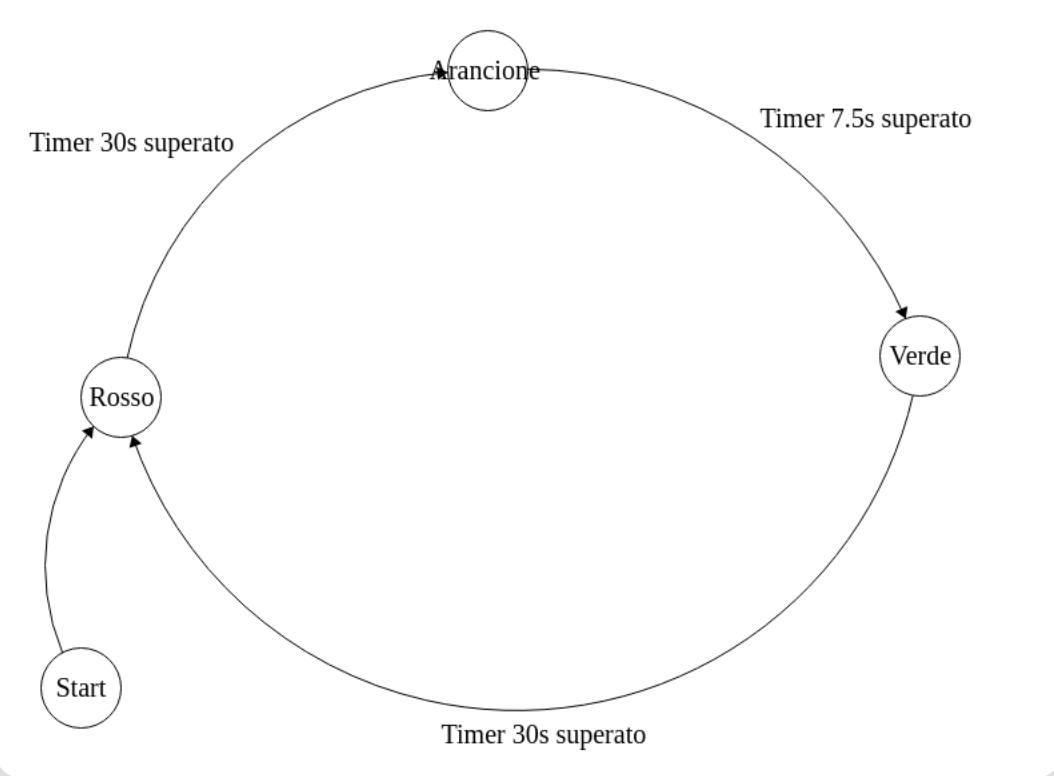
\includegraphics[width=\textwidth]{semaforo.png}
    \end{center}

    PLC: Programmable Logic Controller
    \newline
    Nati per risolvere in modo automatico reti elettriche e automi elettromeccanici.
    \newline
    Da un punto di vista elettronico sono reti combinatorie e automi con flip flop.

    Oggi i TLC sono connessi in rete ma non è necessario che sia così. Originariamente i PLC venivano programmati in un linguaggio
    particolare chiamato KOP o Ladder che si basa sulle porte logiche, interruttori e bobine.

    DSP permettono di eseguire azioni in tempi rapidissimi.

    \section{Progettazione centralina}

    Tutte le combinazioni logiche sono state radunate e influenzano un marker.
    Esiste un contatto SpecialMerker0.0 (SM00) che indica lo stato di accensione e quindi è sempre ON.
    SpecialMerker0.1 (SM01) è ON solo durante il primo ciclo. Ciclo = lettura degli ingressi. Possiamo usarlo per passare allo stato di accensione.

    Per ogni stato serve un flag (ovvero un merker).

    \begin{enumerate}
        \item Merker 0.0 (rete AND)
        \item Merker 1.0 (fermo)
        \item Merker 1.1 (irrigazione)
        \item Merker 1.2 (avaria)
    \end{enumerate}

    5 network per risolvere l'automa + 1 per la rete AND

    \begin{center}
        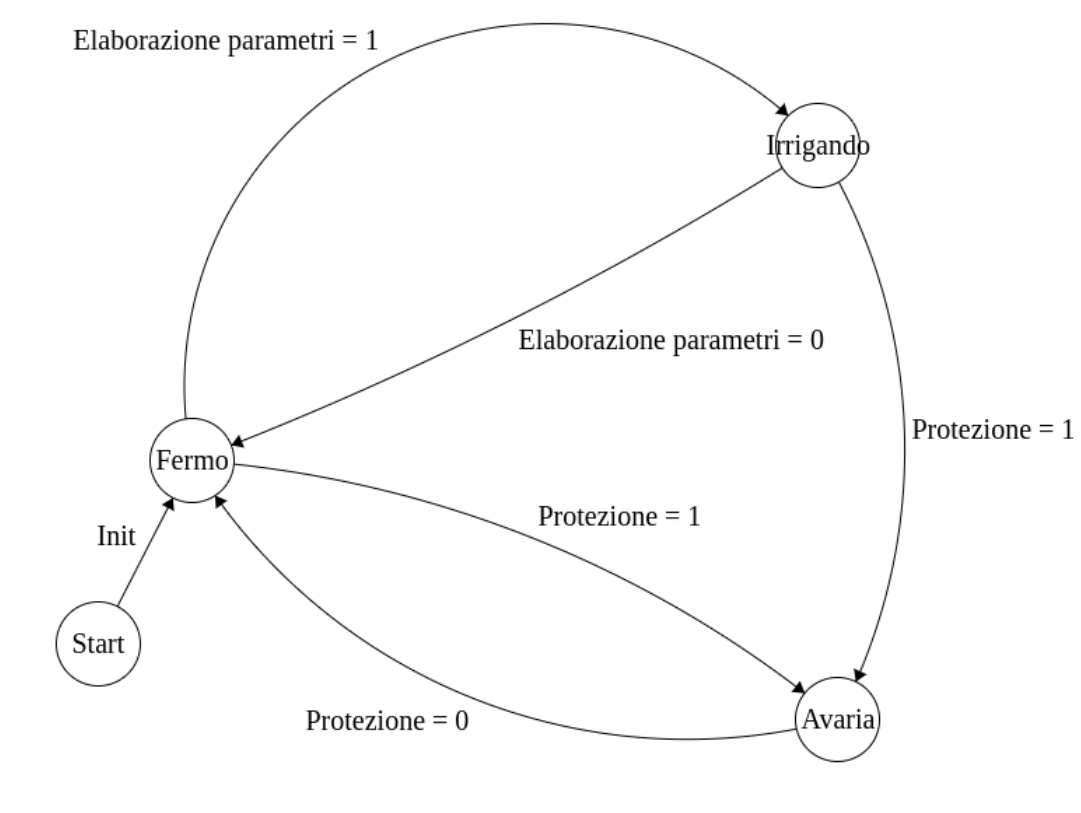
\includegraphics[width=\textwidth]{irrigazione_state.png}
    \end{center}

    (S) = bobina di settaggio

    Ogni volta che cambio lo stato, setto quello nuovo e resetto quello precedente.
    In tutto 6 network.

    Aggiungere anche un allarme acqua che viene attivato quando non c'è abbastanza acqua.

    Tabella di stato (stato -> uscita)
    \begin{enumerate}
        \item Irriga $\rightarrow$ Q1.0
        \item Allarme $\rightarrow$ Q1.1
        \item Livello $\rightarrow$ Q1.2
    \end{enumerate}

    Mettere tutto in bella e consegnare in PDF

    Avaria deve essere sempre su


\end{document}
